\section{SDN-based Static Routing}
\vspace{-2mm}
\subsection*{Static Routing}
Experiment 2에서는 Statical routing을 다룬다. Statical routing에서 packet의 openflow 스위치간의 연결을 
특정경로로 설정을 위해서  각 스위치의 라우팅 테이블을 일일이 입력하는 방법으로 진행된다.
\vspace{-4mm}
\subsection{Construct Static Routing path 1}
\subsubsection*{The Path}
아래와 같은 경로로 Static Routing이 될수 있도록 Flow Table에 Flow를 추가해 주었다.\\
    % \vspace{-2mm}
    % \begin{equation*}
    % \text{h1} \to \text{s1} \to \text{s3} \to \text{s5} \to \text{s6} \to \text{h6} 
    % \end{equation*}
    % \vspace{-2mm}
    \vspace{-4mm}
\begin{figure}[!h]\centering 
	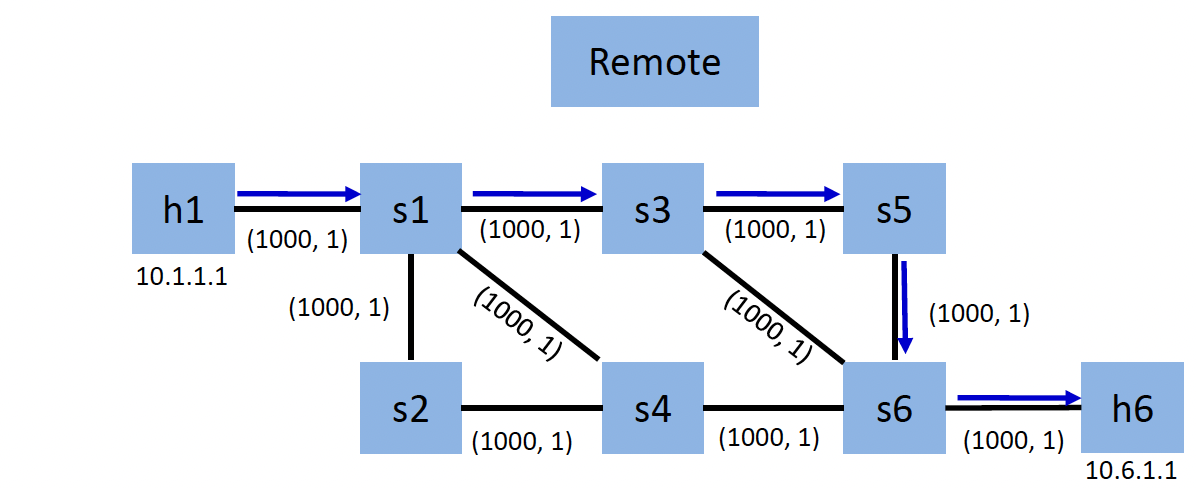
\includegraphics[width=.65\textwidth]{image/week08/2-1-0.png}
% 	\caption{\footnotesize
% 	  }
	\vspace{-10pt}
\end{figure}
\begin{listing}[h!]
\inputminted[framerule = 1pt,framesep = 2mm , frame = lines, fontsize=\footnotesize]{python}{./code/week08/flow2-1.sh}
\vspace{-5mm}
\caption{\footnotesize Experiment 2-1’s dpctl flow-add command}
\end{listing}
    \vspace{-12mm}
\subsubsection*{Flow Table}
\begin{figure}[!h]\centering 
	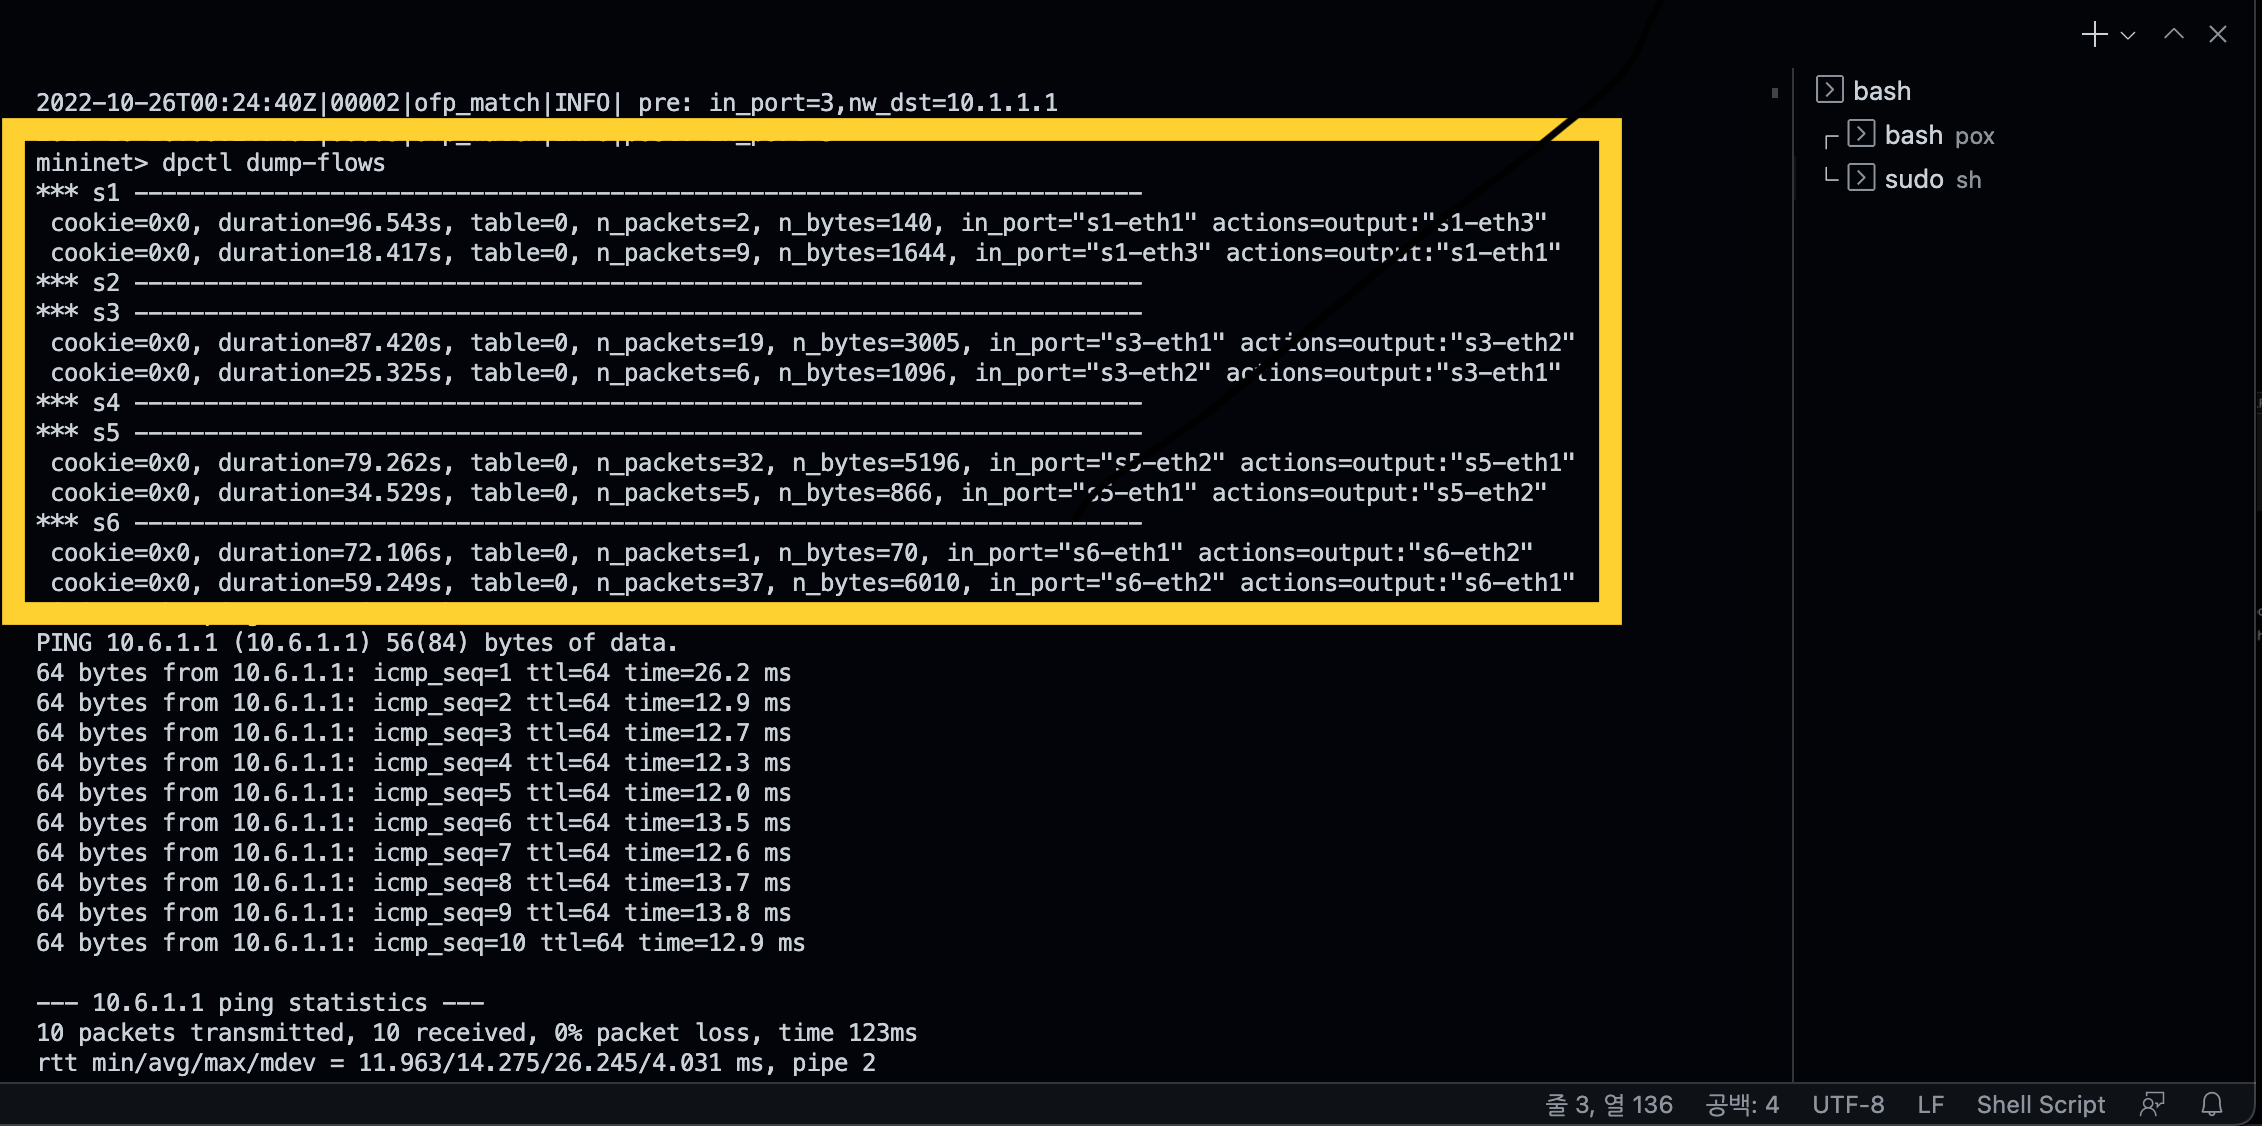
\includegraphics[width=.99\textwidth]{image/week08/2-1-1.png}
	\caption{\footnotesize
	 Experiment 2-1’s flow table}
	\vspace{-10pt}
\end{figure}
\clearpage
\subsubsection*{Ping Test}
\begin{figure}[!h]\centering 
	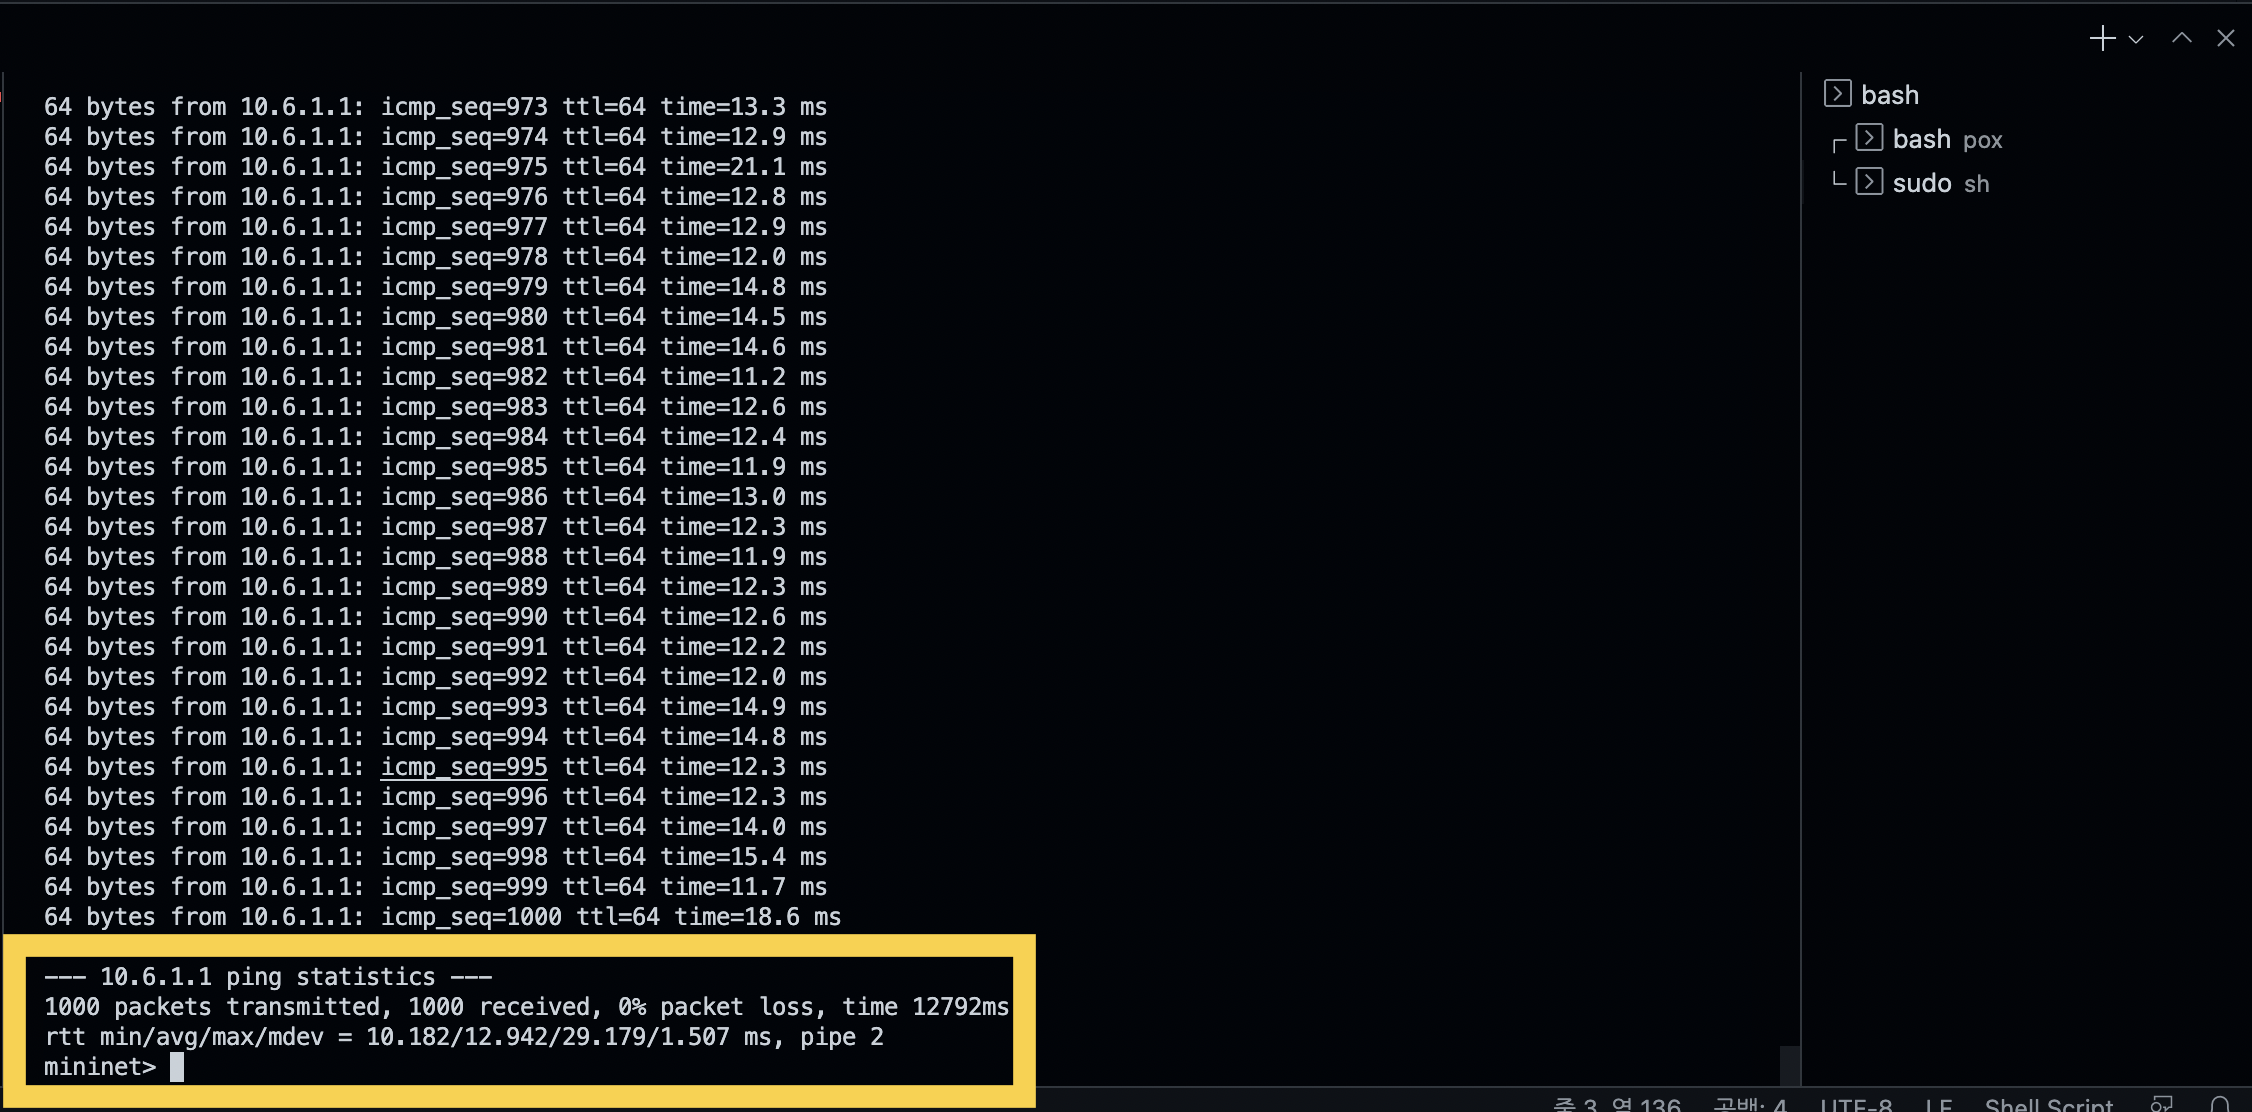
\includegraphics[width=.99\textwidth]{image/week08/2-1-2.png}
	\caption{\footnotesize
	 Experiment 2-1’s pingtest reuslts, $12.944\ ms$, average}
	\vspace{-10pt}
\end{figure}
\subsection{Construct Static Routing path 2}
\subsubsection*{The Path}
아래와 같은 경로로 Static Routing이 될수 있도록 Flow Table에 Flow를 추가해 주었다. 
    \vspace{-2mm}
    \begin{equation*}
    \text{h1}\to\text{s1}\to \text{s3} \to \text{s6}\to\text{h6}
    \end{equation*}
    \vspace{-2mm}
    \vspace{-4mm}
\begin{figure}[!h]\centering 
	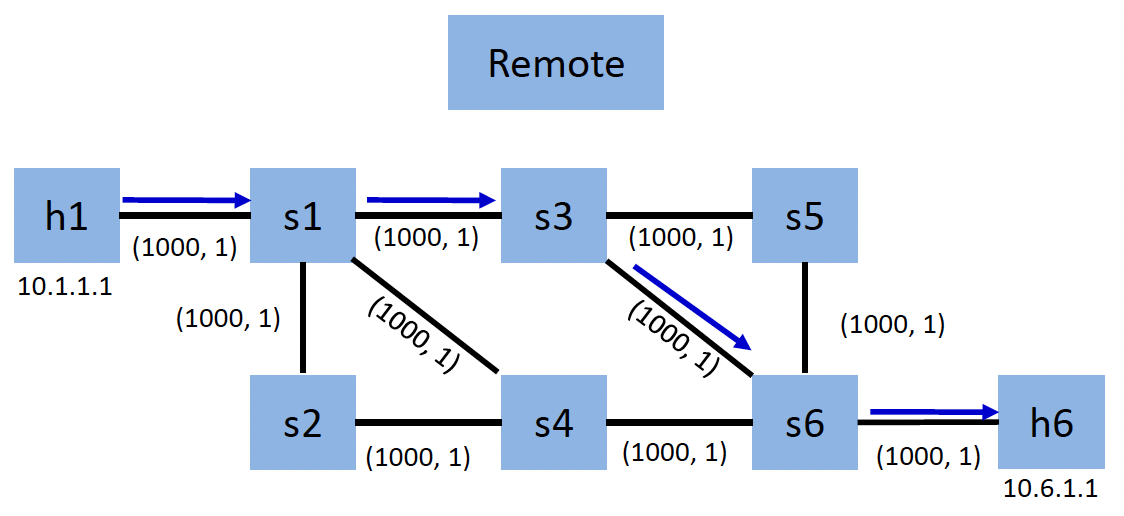
\includegraphics[width=.65\textwidth]{image/week08/2-2-0.png}
	\caption{\footnotesize
	 Experiment 2-1’ Path Diagram}
	\vspace{-10pt}
\end{figure}
\begin{listing}[h!]
\inputminted[framerule = 1pt,framesep = 2mm , frame = lines, fontsize=\footnotesize]{python}{./code/week08/flow2-2.sh}
\vspace{-5mm}
\caption{\footnotesize Experiment 2-2’s dpctl flow-add command}
\end{listing}
\clearpage
    % \vspace{-12mm}
\subsubsection*{Flow Table}
\begin{figure}[!h]\centering 
	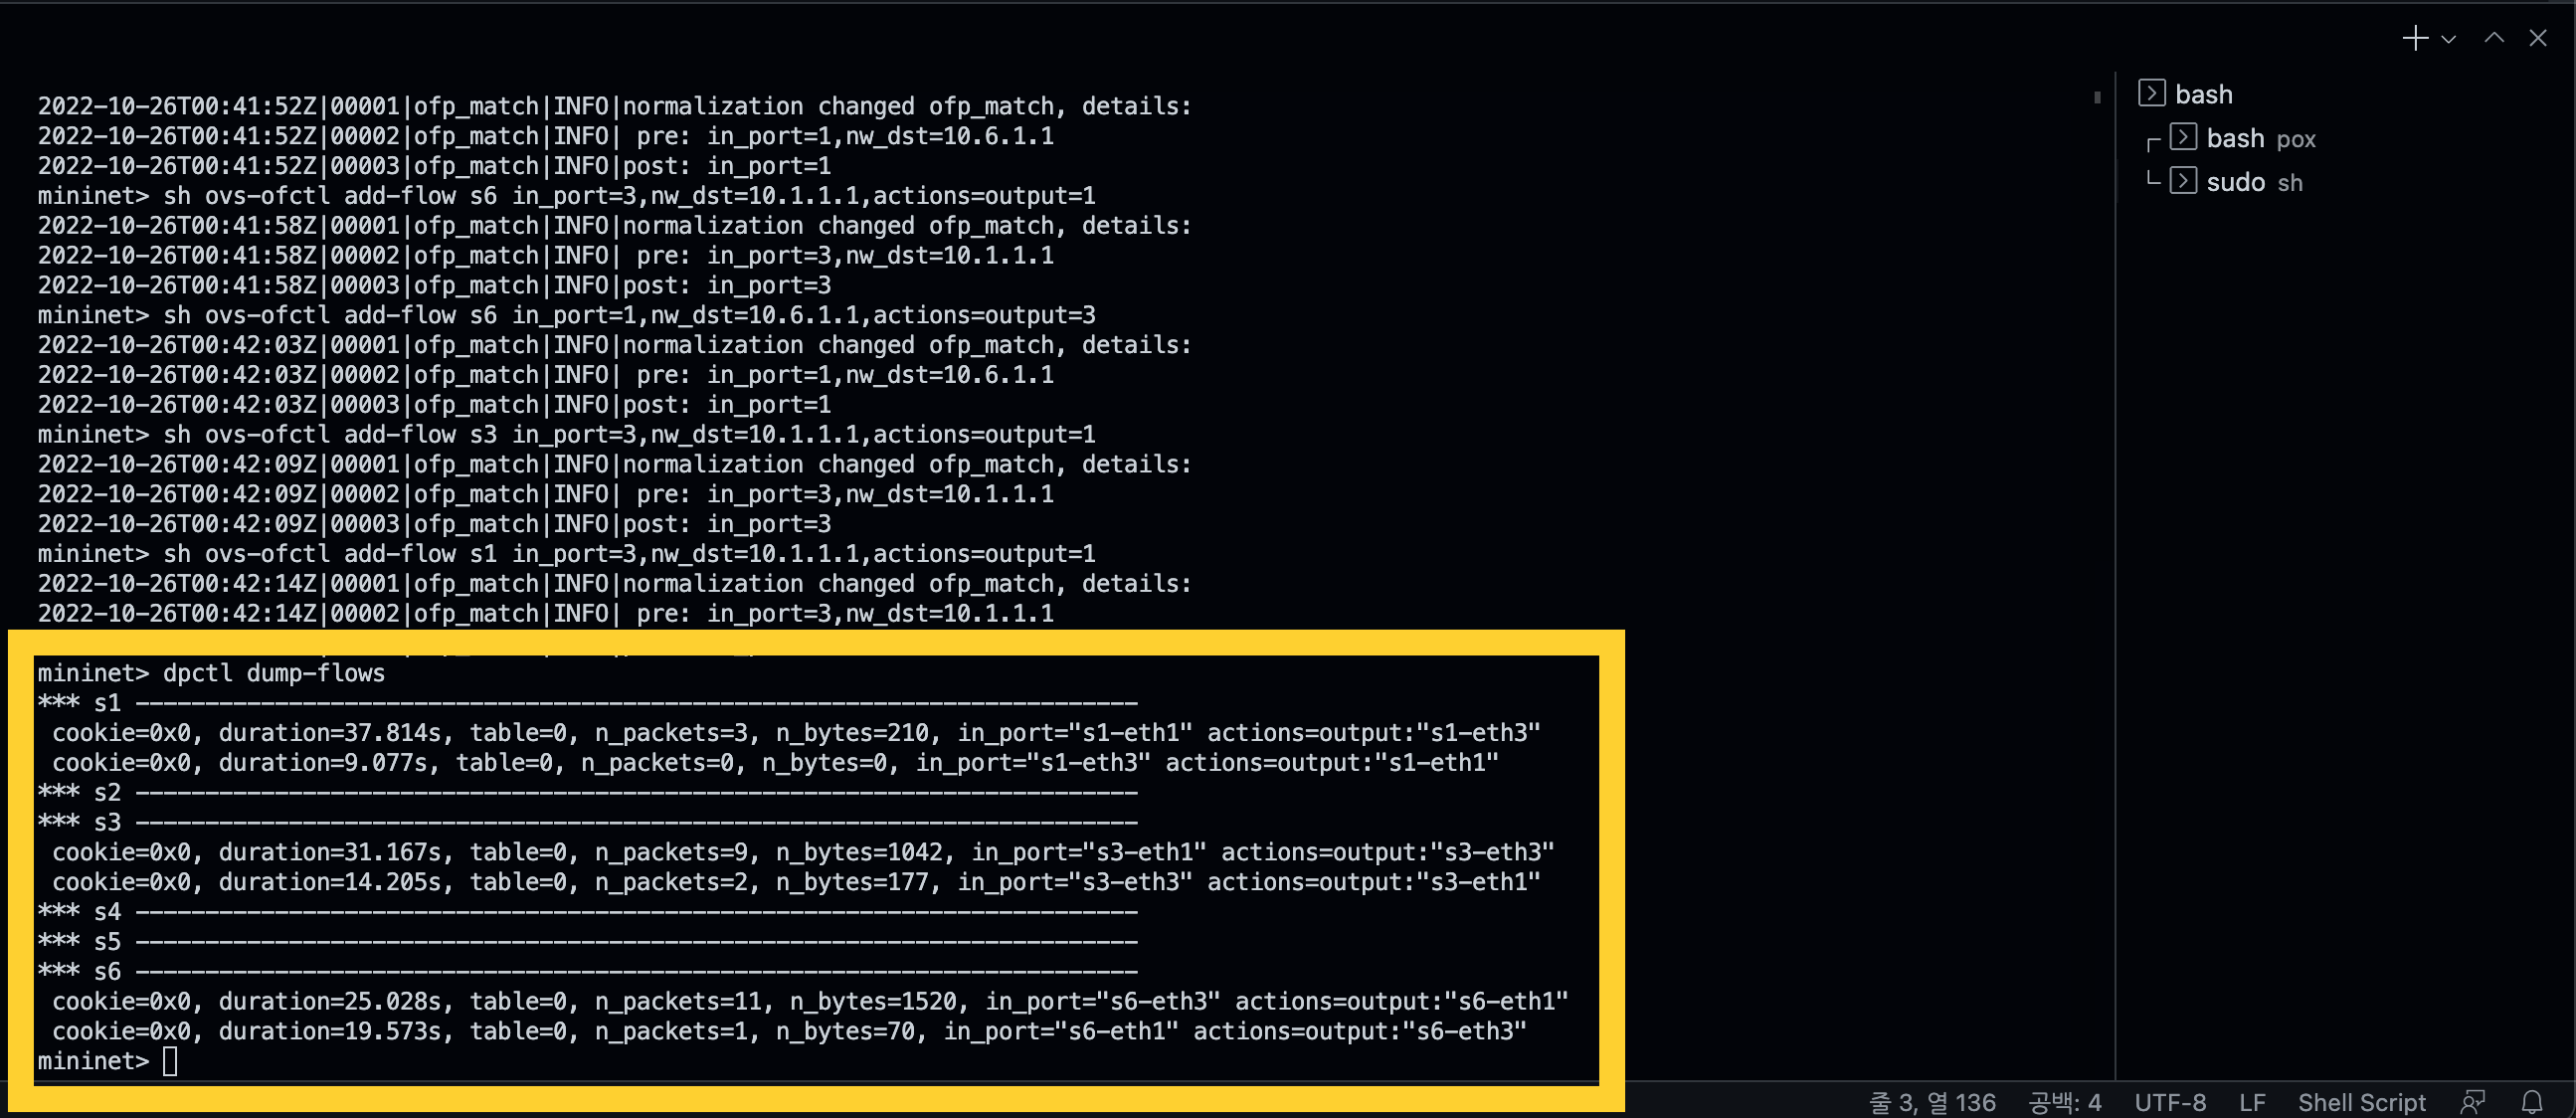
\includegraphics[width=.99\textwidth]{image/week08/2-2-1.png}
	\caption{\footnotesize
	 Experiment 2-1’s flow table}
	\vspace{-10pt}
\end{figure}
\subsubsection*{Ping Test}
Pingtest를 통해서 1000개의 packet의 평균 RTT를 측정한 결과 $10.261\ ms$로,experiment 2-1 에서 측정된 $12.944\ ms$ 보다 짧은 경로라서 값이 줄어든것을 확인할 수 있다.\\
\vspace{-4mm}
\begin{figure}[!h]\centering 
	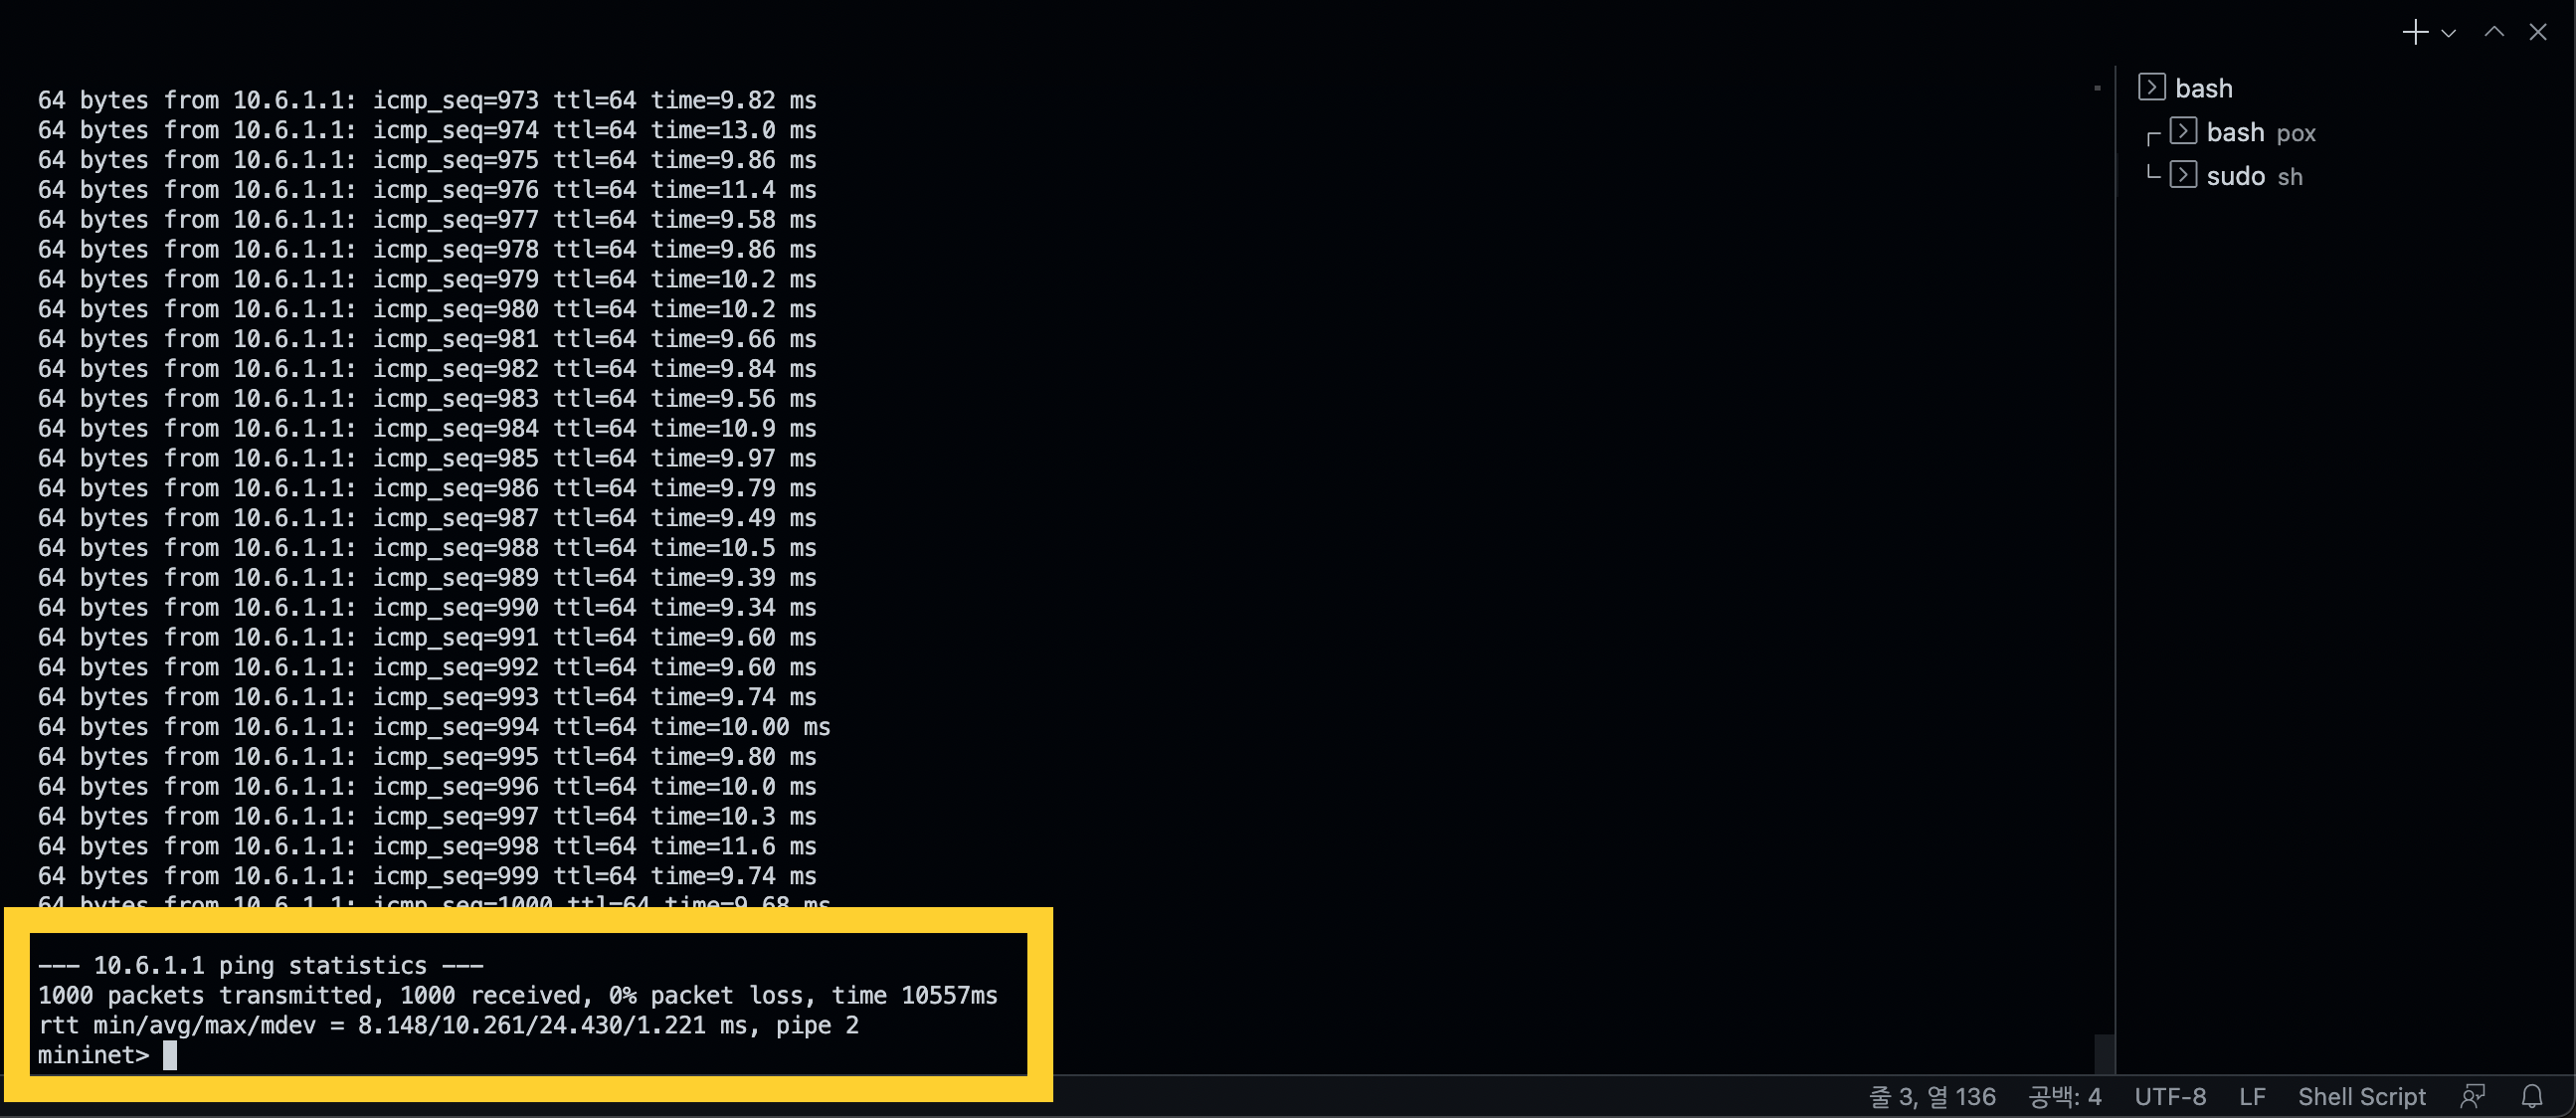
\includegraphics[width=.99\textwidth]{image/week08/2-2-2.png}
	\caption{\footnotesize
	 Experiment 2-1’s pingtest reuslts, $10.261\ ms$, average}
	\vspace{-10pt}
\end{figure}
\clearpage